%% LyX 2.4.0~beta5 created this file.  For more info, see https://www.lyx.org/.
%% Do not edit unless you really know what you are doing.
\documentclass[english]{foils}
\usepackage[T1]{fontenc}
\usepackage[latin9]{inputenc}
\pagestyle{foilheadings}
\setcounter{secnumdepth}{1}
\setcounter{tocdepth}{1}
\usepackage{xcolor}
\usepackage{array}
\usepackage{pifont}
\usepackage{fancybox}
\usepackage{calc}
\usepackage{multirow}
\usepackage{amsmath}
\usepackage{amsthm}
\usepackage{amssymb}
\usepackage{graphicx}
\PassOptionsToPackage{normalem}{ulem}
\usepackage{ulem}

\makeatletter

%%%%%%%%%%%%%%%%%%%%%%%%%%%%%% LyX specific LaTeX commands.
%% Because html converters don't know tabularnewline
\providecommand{\tabularnewline}{\\}

%%%%%%%%%%%%%%%%%%%%%%%%%%%%%% Textclass specific LaTeX commands.
\theoremstyle{definition}
\newtheorem{defn}{\protect\definitionname}
\theoremstyle{definition}
 \newtheorem{example}{\protect\examplename}
\newenvironment{lyxcode}
	{\par\begin{list}{}{
		\setlength{\rightmargin}{\leftmargin}
		\setlength{\listparindent}{0pt}% needed for AMS classes
		\raggedright
		\setlength{\itemsep}{0pt}
		\setlength{\parsep}{0pt}
		\normalfont\ttfamily}%
	 \item[]}
	{\end{list}}
\theoremstyle{remark}
\newtheorem*{rem*}{\protect\remarkname}

%%%%%%%%%%%%%%%%%%%%%%%%%%%%%% User specified LaTeX commands.
\usepackage{xcolor}
\renewcommand{\labelitemi}{$\textcolor{blue}{\bullet}$}
\renewcommand{\labelitemii}{$\textcolor{teal}{\Rightarrow}$}
\renewcommand{\labelitemiii}{$\textcolor{red}{\rightarrow}$}
\renewcommand{\labelitemiv}{$\textcolor{brown}{\circ}$}
% for French theorems, etc. since I'm using English to fix bullet pb.
\providecommand{\examplename}{Example}
\providecommand{\definitionname}{Definition}
\providecommand{\theoremnname}{Theorem}
\providecommand{\remarkname}{Remark}
\providecommand{\exercisename}{Exercise}

\makeatother

\usepackage{babel}
\providecommand{\definitionname}{Definition}
\providecommand{\examplename}{Example}
\providecommand{\remarkname}{Remark}

\begin{document}

\MyLogo{Intro to ML}
\title{Supervised Learning - Linear Regression }
\author{Mark Asch - IMU/VLP/CSU }
\date{2023}
\maketitle

\foilhead{Program}
\begin{enumerate}
\item Data Analysis

\begin{enumerate}
\item Introduction: the 4 identifiers of ``big data'' and ``data science''
\item \textcolor{red}{Supervised learning methods: regression}, k-NN, linear
classification methods, SVM, NN, decision trees. 
\item Unsupervised learning methods: k-means, principal component analysis,
clustering.
\end{enumerate}
\end{enumerate}

\foilhead{The Data Science Process }
\begin{center}
\includegraphics{graphics/DataScienceProcess}
\par\end{center}
\begin{enumerate}
\item Raw\textcolor{magenta}{{} data}: measurements, observations, web-crawling,
etc.
\item Collection and \textcolor{magenta}{cleaning}: pipelines of data munging
with tools such as Python, R, SQL, etc.
\item Exploratory data analysis (\textcolor{magenta}{EDA}).
\item Choice of a \textcolor{magenta}{model} as a function of problem type:
classification, prediction, description

\begin{enumerate}
\item \textcolor{red}{Algorithms of statistical learning}
\item Statistical modeling
\end{enumerate}
\item Interpret, visualize, report, communicate the results (or create an
app !)
\end{enumerate}

\foilhead{Statistical Learning: what is it?}
\begin{center}
\includegraphics[scale=0.35]{graphics/Types-of-Machine-Learning--At-a-Glance-optimized}
\par\end{center}
\begin{defn}
Statistical Learning (``machine learning'') is a collection of tools
for understanding data by seeking relations between them.
\end{defn}
The tools can be classified into:
\begin{itemize}
\item \textcolor{magenta}{supervised} tools, where we construct a statistical
model to predict or estimate an \emph{output}, based on \emph{inputs;}
\item \textcolor{magenta}{unsupervised} tools, where we learn relations
among \emph{inputs} without any outputs (response variables) that
supervise;
\item tools for \textcolor{magenta}{reinforcement} learning, where an agent
learns the environment by interacting with it, and by receiving rewards
(process of maximization of the expected cumulative reward)
\end{itemize}

\foilhead{Supervised and Unsupervised}

\includegraphics[scale=1.5]{\string"graphics/Pages from Pages from 01_Introduction-5\string".pdf}

\foilhead[-0.5in]{Which model for which task? }

\begin{tabular}{|c|c|c|}
\hline 
Class & Model & Task\tabularnewline
\hline 
\hline 
\multirow{6}{*}{Supervised} & linear regression & R\tabularnewline
\cline{2-3}
 & CART (trees) & R\&C\tabularnewline
\cline{2-3}
 & SVM & R\&C\tabularnewline
\cline{2-3}
 & NN & R\&C\tabularnewline
\cline{2-3}
 & $k$-NN & C\tabularnewline
\cline{2-3}
 & Naive Bayes & C\tabularnewline
\hline 
\multirow{3}{*}{Unsupervised} & $k$-means & Clustering\tabularnewline
\cline{2-3}
 & dendrogram & Clustering\tabularnewline
\cline{2-3}
 & PCA & pattern\tabularnewline
\hline 
\end{tabular}

R = regression, C = classification

\foilhead{Recall: the mathematical framework}
\begin{itemize}
\item Suppose that we have:

\begin{itemize}
\item a \textcolor{magenta}{response} variable (to explain), $Y$,
\item $p$ \textcolor{magenta}{explanatory}\footnote{\textcolor{magenta}{Also called: features, attributes}}\textcolor{magenta}{{}
}variables, $X=(X_{1},X_{2},\ldots,X_{p})$,
\item a relationship between $Y$ and $X$ of the form
\[
Y=f(X)+\epsilon
\]
\item where

\begin{itemize}
\item $f$ is an \textcolor{magenta}{unknown} function of $X_{1},X_{2},\ldots,X_{p}$
\item $\epsilon$ is a random \textcolor{magenta}{error} term, independent
of $X,$ and with zero mean
\end{itemize}
\end{itemize}
\item ML is then an ensemble of approaches for \textcolor{magenta}{estimating}
$f$ with the objectives of 

\begin{itemize}
\item \textcolor{magenta}{Prediction}: $\hat{Y}=\hat{f}(X)$ where $\hat{f}$
is an estimation for $f$ and $\hat{Y}$ is the resulting prediction
\item \textcolor{magenta}{Inference}: to understand how $Y$ varies as a
function of $X$ (correlations, importances, linearity, etc.)
\end{itemize}
\end{itemize}

\foilhead{Errors}
\begin{example}
Let $X_{1},X_{2},\ldots,X_{p}$ be characteristics of a patient's
blood sample, easily measured in a laboratory. Let $Y$ be a variable
that describes the patient's risk of an adverse reaction to a given
drug. It is natural to seek to predict $Y$ from $X$ - then we can
avoid to give the drug to high-risk patients.
\end{example}
The precision of $\hat{Y}$ as a prediction of $Y$ depends on 2 quantities:
\begin{itemize}
\item the \textcolor{magenta}{reducible} error - $\hat{f}$ is not a perfect
estimate $f$ and can be improved
\item the \textcolor{magenta}{irreducible} error - $\epsilon$ cannot be
predicted by $f$ ($\epsilon$ can contain effects of non-measured
variables - for example, the risk of an adverse reaction can depend
on the patient's health status on the given day, or the variability
in the manufacture of the drug)
\end{itemize}
We can show that
\begin{align*}
E(Y-\hat{Y})^{2} & =E\left[f(X)+\epsilon-\hat{f}(X)\right]^{2}\\
 & =\underbrace{\left[f(X)-\hat{f}(X)\right]^{2}}+\underbrace{\mathrm{Var}(\epsilon)}\\
 & \qquad\quad\mathrm{reducible}\mathrm{\qquad irreducible}
\end{align*}

\begin{dinglist}{52}
\item The objective of Statistical Leaning is to study techniques for the
estimation of $f$ while \textcolor{magenta}{minimizing the reducible
error}... 
\end{dinglist}

\foilhead{Regression and Classification}

Variables can be characterized as:
\begin{dinglist}{52}
\item \textcolor{magenta}{quantitative}, taking on numerical values
\item \textcolor{magenta}{qualitative} (or categorical), that take values
in one of $K$ different classes (or categories).
\end{dinglist}
The problems are then of type:
\begin{dinglist}{52}
\item \textcolor{magenta}{regression} when we have quantitative variables,
\item \textcolor{magenta}{classification} for qualitative variables.
\end{dinglist}
\includegraphics[scale=1.25]{\string"graphics/Pages from Pages from 01_Introduction-8\string".pdf}

\includegraphics[scale=1.25]{\string"graphics/Pages from Pages from 01_Introduction-8-2\string".pdf}
\begin{itemize}
\item the only difference is the space in which $y_{i}$ takes its values:
\begin{itemize}
\item continuous space, $\mathbb{R}^{n},$ for regression
\item discrete space, $\mathbb{N}^{n},$ for classification
\end{itemize}
\end{itemize}

\foilhead{Linear Regression }

\textbf{\textcolor{red}{Hypothesis}} : there exists a \textcolor{magenta}{linear}
relation between the output (response, dependent) variable and the
input (explanatory, independent, feature) variable(s)
\begin{dinglist}{52}
\item LR is one of the most widely-used statistical learning methods 
\item LR implies a linear correlation between the changes in an explanatory
variable and its output
\end{dinglist}
We start with \textcolor{magenta}{simple linear regression} (SLR)
: 
\[
Y\approx\beta_{0}+\beta_{1}X
\]
where
\begin{itemize}
\item $\beta_{0}$ is the intercept and $\beta_{1}$ is the slope;
\item $\left\{ \beta_{0},\beta_{1}\right\} $ are the \textcolor{magenta}{parameters}
of the model that we will estimate by $\left\{ \hat{\beta}_{0},\hat{\beta}_{1}\right\} $ 
\end{itemize}
We obtain the \textcolor{magenta}{prediction model}
\[
\hat{y}=\hat{\beta}_{0}+\hat{\beta}_{1}x
\]


\foilhead{Estimating the parameters}
\begin{itemize}
\item In practice, $\beta_{0}$ and $\beta_{1}$ are \textcolor{magenta}{unknown}
\item We must use the data to estimate the coefficients...
\item Let the \textcolor{magenta}{observations }be
\[
(x_{1},y_{1}),\,\,(x_{2},y_{2}),\,\,\cdots,(x_{n},y_{n})
\]
\item Our objective: obtain the\textcolor{magenta}{{} best fit} possible between
a linear model and the data
\item We will use\textcolor{magenta}{{} the least squares criterion} (there
are others... see lecture on ``Other Regression Methods'')
\end{itemize}

\foilhead{Least Squares}
\begin{defn}
The residue of the $i$-th response is
\[
e_{i}=y_{i}-\hat{y}_{i}
\]
and the sum of squares of residues is defined by
\begin{align*}
\mathrm{RSS}(\beta) & =e_{1}^{2}+e_{2}^{2}+\cdots+e_{n}^{2}\\
 & =\sum_{i=1}^{n}\left(y_{i}-\hat{\beta}_{0}-\hat{\beta}_{1}x_{i}\right)^{2}
\end{align*}
\end{defn}
\noindent\shadowbox{\begin{minipage}[t]{1\columnwidth - 2\fboxsep - 2\fboxrule - \shadowsize}%
The\textcolor{magenta}{{} least squares criterion}: choose $\hat{\beta}_{0}$
and $\hat{\beta}_{1}$ to minimize the $\mathrm{RSS}.$%
\end{minipage}}

\foilhead{Coefficients of SLR}
\begin{dinglist}{52}
\item To minimize the RSS, we differentiate with respect to $\beta$ and
we set the derivatives equal to zero\footnote{This is known as the ``necessary condition for optimality''. }...
\begin{align*}
\hat{\beta}_{1} & =\frac{\sum_{i=1}^{n}\left(x_{i}-\bar{x}\right)\left(y_{i}-\bar{y}\right)}{\sum_{i=1}^{n}\left(x_{i}-\bar{x}\right)^{2}}=\frac{s_{xy}}{s_{x}^{2}}\\
\hat{\beta}_{0} & =\bar{y}-\hat{\beta}_{1}\bar{x}
\end{align*}
where 
\[
\bar{x}=\frac{1}{n}\sum_{i=1}^{n}x_{i}\qquad\mathrm{and}\qquad\bar{y}=\frac{1}{n}\sum_{i=1}^{n}y_{i}
\]
are the \textcolor{magenta}{empirical averages}.
\end{dinglist}

\foilhead[-0.5in]{How to do this with \textcolor{blue}{R}?}
\begin{center}
\includegraphics[height=0.9\textheight]{/Users/markasch/Dropbox/3Teaching/stat-ML/Master-ISC/02TD-TP/SLR}
\par\end{center}

\foilhead[-0.5in]{How to do this with \textcolor{blue}{Python} (statsmodels)?}
\begin{center}
\includegraphics[height=0.8\textheight]{/Users/markasch/Dropbox/3Teaching/stat-ML/Master-ISC/02TD-TP/SLRpy}
\par\end{center}

\foilhead[-0.5in]{How to do this with \textcolor{blue}{Python} (sklearn)?}
\begin{center}
\includegraphics[height=0.8\textheight]{/Users/markasch/Dropbox/3Teaching/stat-ML/Master-ISC/02TD-TP/SLRsk-2}
\par\end{center}

\foilhead{SLR: Analysis of results}
\begin{itemize}
\item The estimated straight line is
\[
\hat{y}=-116,23+49,24\,x
\]
\item But, if a new measurement arrives, with an $x$-value of $5,$ with
what\textcolor{magenta}{{} confidence} can we claim that the response
is
\[
-116,23+49,24\,*\,5=129,97\;?
\]
\item For this, we need to \textcolor{magenta}{extend the model} by:

\begin{dinglist}{52}
\item Adding hypotheses of error modeling.
\item Adding predictive variables.
\item Transforming the predictive variables. 
\end{dinglist}
\end{itemize}

\foilhead[-0.5in]{I. Error Modeling Hypotheses}
\begin{itemize}
\item If we use a model to predict $y$ for a given value $x,$ then the
prediction is \textcolor{magenta}{deterministic} and does not take
into account the variability in the observed data...
\item We generalize the model to
\[
y=\beta_{0}+\beta_{1}x+\epsilon,
\]
where the new term $\epsilon$ is a random ``noise'' and is called
the \textcolor{magenta}{error }term
\item Modeling hypotheses on $\epsilon$ are:

\begin{itemize}
\item the error follows a \textcolor{magenta}{Gaussian} distribution, with
zero mean and variance $\sigma,^{2}$that is $\epsilon\sim\mathcal{N}\left(0,\sigma^{2}\right)$ 
\item the error is \textcolor{magenta}{independent} of $x$ and
\item the errors $\epsilon_{i}$ are uncorrelated and of equal variance
(i.i.d.)
\end{itemize}
\item Mathematically, the model tells us that for any given value of $x,$
the \textcolor{magenta}{conditional distribution} of $y$ for $x$
given, is
\[
p\left(y\vert x\right)\sim\mathcal{N}\left(\beta_{0}+\beta_{1}x,\sigma^{2}\right)
\]
\end{itemize}

\foilhead{Noise Model}
\begin{itemize}
\item A noise model is essential for any analysis, particularly \textcolor{magenta}{Bayesian}
(of which regression is an example)
\item \textcolor{magenta}{Neutrality} of the Gaussian hypothesis for the
noise model:
\begin{itemize}
\item the noise is centered : its mean value is zero, but it can take any
value (small or big)
\item large amplitudes/deviations are less and less probables: the variance
is finite
\item independence between observations (otherwise, this is part of the
trends of the model)
\end{itemize}
\item We neither suppose, nor impose that the noise really follows a Gaussian
law...
\end{itemize}

\foilhead{Estimation of parameters}
\begin{itemize}
\item How do we \textcolor{magenta}{fit} such a model? How do we compute
the parameters $\beta_{0},$ $\beta_{1}$ and $\sigma$ from the data?
\item \textcolor{red}{Theorem}: the least squares estimate for $\beta_{0},$
$\beta_{1}$ is optimal, being unbiased and of minimal variance (
\textcolor{blue}{BLUE} estimator)
\item Estimation of the \textcolor{magenta}{variance} : the mean squared
error, defined by
\[
\mathrm{MSE}=\frac{\sum_{i=1}^{n}e_{i}^{2}}{n-2}=\frac{\mathrm{RSS}}{n-2}
\]
(quantifies the variation of the predicted value with respect to the
observation) is an \textcolor{magenta}{unbiased estimator} of the
variance $\sigma^{2}.$
\item But how can we measure the \textcolor{magenta}{confidence} ?
\end{itemize}

\foilhead{Evaluation metrics for SLR}
\begin{dinglist}{52}
\item In the output of the function \texttt{\textcolor{blue}{lm}} of \texttt{\textcolor{blue}{R}}
: \textcolor{magenta}{p-value} and\textcolor{magenta}{{} R-squared}
\end{dinglist}
\begin{lyxcode}
{\small >~summary(model)}{\small\par}

{\small Call:~lm(formula~=~y~\textasciitilde ~x)}{\small\par}

{\small Residuals:~~~~~~~1~~~~~~~2~~~~~~~3~~~~~~~4~~~~~~~5~~~~~~~6~~~}{\small\par}

{\small ~~~~~~~~~~~~~~47.547~~11.507~~~1.267~-43.213~~40.827~-57.933~}{\small\par}

{\small Coefficients:~~~~~~}{\small\par}

{\small ~~~~~~~~~~~~~Estimate~Std.~Error~t~value~Pr(>|t|)}{\small\par}

{\small (Intercept)~-116.227~~~~~54.792~~-2.121~~0.10120~~~~}{\small\par}

{\small x~~~~~~~~~~~~~49.240~~~~~~7.868~~~6.258~~0.00332~{*}{*}~}{\small\par}

{\small -{}-{}-~}{\small\par}

{\small Signif.~codes:~~0~\textquoteleft {*}{*}{*}\textquoteright{}~0.001~\textquoteleft {*}{*}\textquoteright{}~0.01~\textquoteleft {*}\textquoteright{}~0.05~\textquoteleft .\textquoteright{}~0.1~\textquoteleft{}~\textquoteright{}~1}{\small\par}

{\small Residual~standard~error:~48.18~on~4~degrees~of~freedom~}{\small\par}

{\small Multiple~R-squared:~~0.9073,~~Adjusted~R-squared:~~0.8842~~}{\small\par}

{\small F-statistic:~39.17~on~1~and~4~DF,~~p-value:~0.003325}{\small\par}
\end{lyxcode}

\foilhead{\textcolor{black}{R-squared }}
\begin{defn}
The \textcolor{red}{proportion of the error}/variance explained by
the model is
\[
R^{2}=1-\frac{\sum_{i}\left(y_{i}-\hat{y}_{i}\right)^{2}}{\sum_{i}\left(y_{i}-\bar{y}\right)^{2}}=1-\frac{\mathrm{RSS}}{\mathrm{TSS}}=\frac{\mathrm{TSS}-\mathrm{RSS}}{\mathrm{TSS}},
\]
where $\mathrm{TSS}$ is the \textcolor{red}{total sum of squares}
that measures the inherent variability in the response before the
regression is done.
\end{defn}
\begin{rem*}
$R^{2}$ (\textcolor{magenta}{coefficient of determination}) measures
the proportion of the variability in $y$ that can be explained using
$x.$ $\mathrm{RSS},$ by contrast, measures the quantity of variability
in the response that is left unexplained after performing the regression.
$\mathrm{TSS}-\mathrm{RSS}$ measures the quantity of variability
that is explained (or removed) by performing the regression.
\end{rem*}

\foilhead{~}
\begin{dinglist}{52}
\item A value of $R^{2}$ close to zero indicates that the regression has
not explained/captured much of the variability in the response...

\begin{dinglist}{52}
\item either a linear model is not suitable,
\item or the inherent $\sigma^{2}$ is too high,
\item or both.
\end{dinglist}
\item \textcolor{red}{Warning} : the value itself of $R^{2}$ is not always
reliable, and the MSE should also be taken into account---see examples
in \texttt{\textcolor{blue}{R-squared-dangers.html}}
\end{dinglist}
\[
\mathrm{MSE}=\frac{1}{n}\sum_{i=1}^{n}\left(y_{i}-\hat{y}_{i}\right)^{2}
\]


\foilhead{\xout{p-Value}}
\begin{itemize}
\item The estimations of $\beta$ can be found in the column ``Estimate''
\item The p-values are in the column, Pr(>ItI)
\end{itemize}
\begin{defn}
The \textcolor{red}{p-value} is the probability, under the null hypothesis
($\beta_{1}=0$), to observe a value greater than $\left|t\right|,$
where the $t$-statistic is given by 
\[
t=\frac{\hat{\beta}_{1}-0}{\mathrm{SE}\left(\hat{\beta}_{1}\right)}
\]
 with standard error, 
\[
\mathrm{SE}\left(\hat{\beta}_{1}\right)^{2}=\frac{\sigma^{2}}{\sum_{i}\left(x_{i}-\bar{x}\right)^{2}}.
\]
\end{defn}

\foilhead{\xout{Interpretation of the p-values}}
\begin{itemize}
\item If the \textcolor{magenta}{p-value is low} (threshold that is context-dependent...),
it is very unlikely to observe such a test statistic under the null
hypothesis (where no trend is supposed)

\begin{itemize}
\item it is this highly probable that the coefficient is non-zero and thus
\textcolor{magenta}{significant} (statistically speaking).
\end{itemize}
\item If the \textcolor{magenta}{p-value is high} we cannot reject the null
hypothesis, since the observed value of the test statistic is probably
not due exclusively to chance (resulting from the intrinsic variability)

\begin{itemize}
\item the coefficient could be zero and non-significant
\end{itemize}
\end{itemize}

\foilhead{Graphical diagnostics}
\begin{itemize}
\item Let the linear model be:\texttt{\textcolor{blue}{{} }}~\\
\texttt{\textcolor{blue}{try <- lm(Amax \textasciitilde{} SLA, data=photo,
na.action=na.omit) }}
\item The command \texttt{\textcolor{blue}{plot(try)}} displays 4 plots:
\begin{enumerate}
\item The plots (``Residuals vs Fitted'' and ``Scale-Location'') should
not give any clear trends (they should neither be all increasing or
all decreasing). This shows, 
\begin{enumerate}
\item that on average, the regression line is well fitted to the data, and
thus the hypothesis of linearity is acceptable,
\item that the variance is constant and of the same value for all the observations.
\end{enumerate}
\item The ``normal Q-Q'' plot should show points distributed around the
dashed line and that follow the line approximately, without marked
deviations (especially at the extremities). This shows that the hypothesis
of the residues having a normal distribution, is satisfied.
\item The last ``Cook distances'', should not show any point that exceeds
1 on the abscissa. This shows the presence of influential data.
\end{enumerate}
\end{itemize}
\begin{center}
\includegraphics[width=1\textwidth]{../../../02course-advanced/01Lessons/01_SciML/graphics/lin_reg_assump}
\par\end{center}

\begin{center}
\includegraphics[width=1\textwidth]{../../../02course-advanced/01Lessons/01_SciML/graphics/LRassumps}
\par\end{center}

\foilhead{Simple Linear Regression Model}
\begin{itemize}
\item \textbf{L}inear Function: The mean of the response, $\mbox{E}(Y_{i}),$
at each value of the predictor, $x_{i},$ is a Linear function of
the $x_{i}.$ 
\item \textbf{I}ndependent: The errors, $\epsilon_{i},$ are Independent.
\item \textbf{N}ormally Distributed: The errors, $\epsilon_{i},$ at each
value of the predictor, $x_{i},$ are Normally distributed.
\item \textbf{E}qual variances (denoted $\sigma^{2}$ ): The errors, $\epsilon_{i},$
at each value of the predictor, $x_{i},$ have Equal variances (denoted
$\sigma^{2}$ ).
\end{itemize}

\foilhead{Cross Validation }
\begin{dinglist}{52}
\item A learning approach, used systematically, for model evaluation...
(see lecture ``Other methods'' for full details)
\end{dinglist}
\begin{itemize}
\item \textcolor{magenta}{Divide/Split} the data into:

\begin{itemize}
\item a\textcolor{magenta}{{} training} subset (80\%)
\item a \textcolor{magenta}{test} subset (20\%)
\end{itemize}
\item \textcolor{magenta}{Fit} the model to the training subset
\item Calculate the \textcolor{magenta}{mean-squared error }on the test
subset
\item \textcolor{magenta}{Compare} with that of the training subset
\item Vary the \textcolor{magenta}{sample size} and repeat.
\end{itemize}

\foilhead{II. Adding predictive variables }
\begin{itemize}
\item We have so far studied\textcolor{magenta}{{} simple linear regression}
with

\begin{itemize}
\item 1 output
\item 1 predictor
\end{itemize}
\item We can easily \textcolor{magenta}{extend this model} by adding predictive
variables,
\[
y=\beta_{0}+\beta_{1}x_{1}+\beta_{2}x_{2}+\beta_{3}x_{3}+\epsilon
\]
\item The model is now called \textcolor{red}{multiple linear regression}.
\item Key idea to \textcolor{magenta}{construct the model}: 

\begin{itemize}
\item plot all \textcolor{magenta}{scatterplots} of $y$ against each of
the predictive variables 
\item plot all \textcolor{magenta}{histograms} of $y\vert x$ for different
values of each predictive variable 
\end{itemize}
\item Evaluation (as before) :

\begin{itemize}
\item $R^{2},$ \textcolor{gray}{p-values}
\item training and test subsets
\end{itemize}
\end{itemize}

\foilhead{III. Transformation of predictive variables }
\begin{itemize}
\item Why suppose a linear relation?
\item Possible to test other relations (non linear) 

\begin{itemize}
\item by defining, for example, $z=x^{2}$
\item then performing a linear regression on $z$
\end{itemize}
\end{itemize}
\begin{dinglist}{56}
\item The biggest challenge is that we never know the ``truth''!
\end{dinglist}

\foilhead{Over- and Under-fitting and the Bias-Variance Tradeoff}
\begin{itemize}
\item A general rule (theorem...) states that by \textcolor{magenta}{reducing
the bias} of a model (by adding variables or parameters), we \textcolor{magenta}{increase
its variance}, which implies greater estimation errors and a rigidity/fragility
of the model obtained.
\item We seek then, in the parametrization of our statistical models, a
\textcolor{magenta}{compromise} between the bias and the variance.
\end{itemize}
\begin{center}
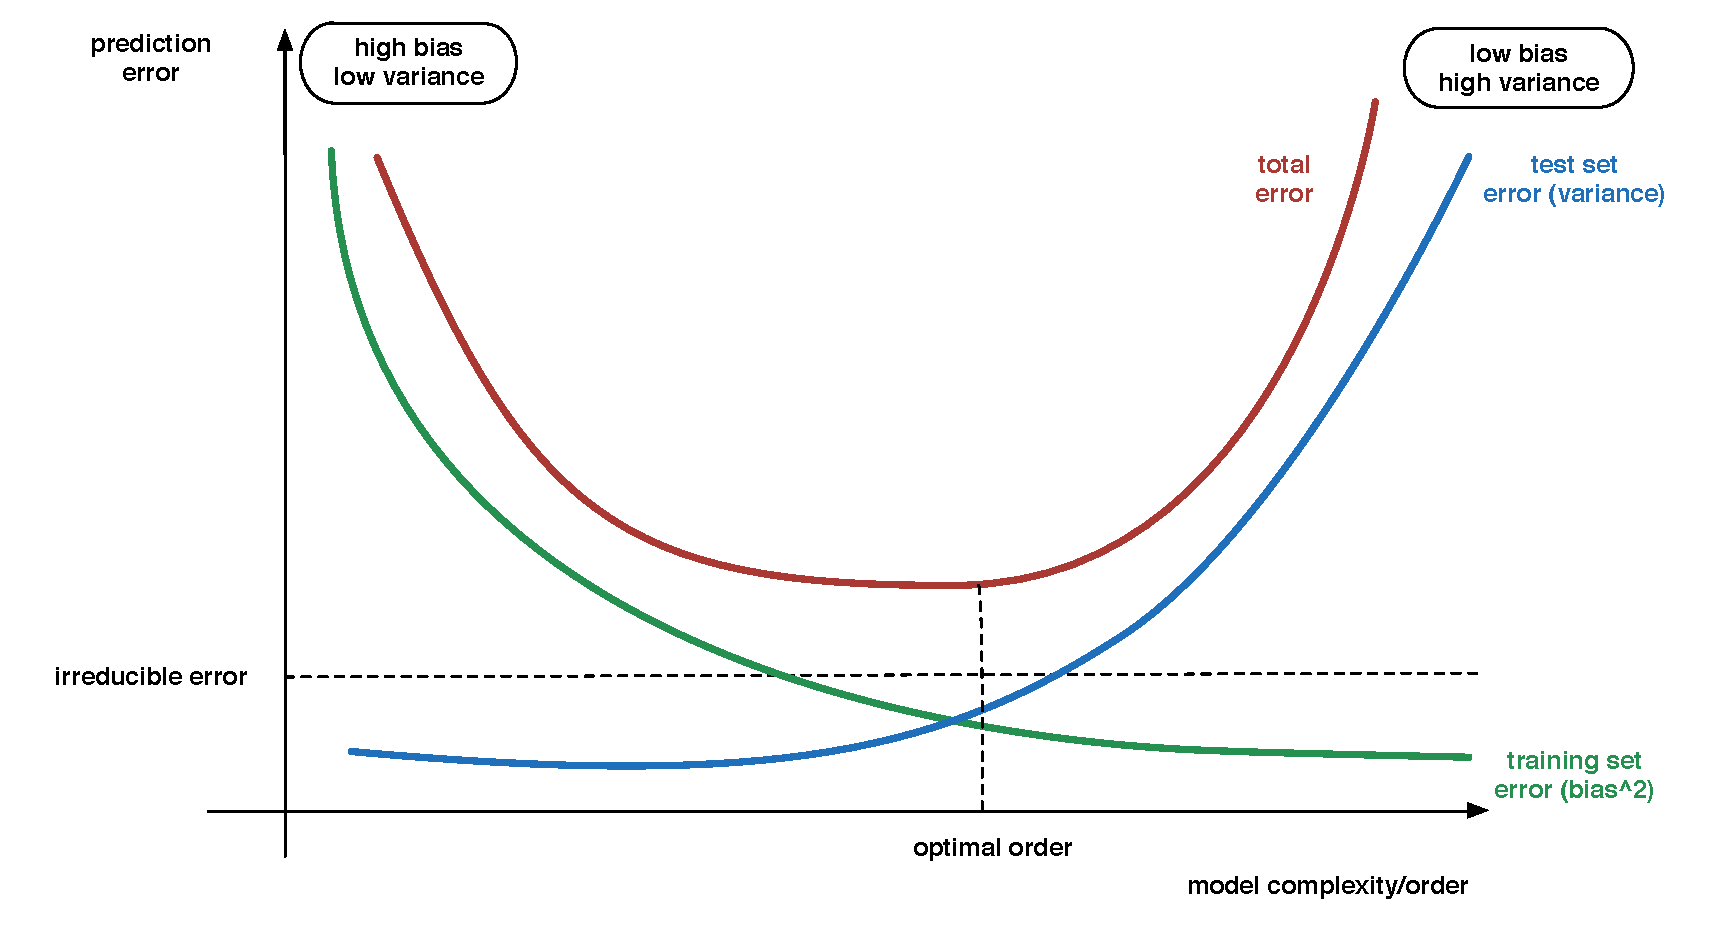
\includegraphics[scale=0.5]{graphics/bias-variance}
\par\end{center}

\foilhead{Example of Regression of a Cosine}
\begin{center}
\includegraphics[width=1\textwidth]{graphics/under-over-regression}
\par\end{center}

\foilhead{References}
\begin{enumerate}
\item M. DeGroot, M. Schervish, \emph{Probability and Statistics}, Addison
Wesley, 2002.
\item Spiegel, Murray and Larry Stephens,\emph{ Schaum's Outline of Statistics,}
6th edition, McGraw Hill. 2017.
\item G. James, D. Witten, T. Hastie, R. Tibshirani. \emph{An Introduction
to Statistical Learning with Applications in R.} Springer. 2013.
\item Rachel Schutt and Cathy O\textquoteright Neil. \emph{Doing Data Science.}
O'Reilly. 2014.
\end{enumerate}

\end{document}
